\documentclass{article}
\usepackage{tikz}
\usetikzlibrary{arrows}
\usepackage{amsmath}
\usepackage[english]{babel}
\usepackage[utf8]{inputenc}
\usepackage{fancyhdr}
 
\pagestyle{fancy}
\fancyhf{}
\rhead{Austin Bursey , Aaron Exley\\ Tim McGill, Joseph Myc}
\lhead{CP468 A1 Group 7\\October 4th 2019}
\rfoot{Page \thepage}

\begin{document}

\begin{titlepage}
  \pagestyle{fancy}
  \thispagestyle{fancy}
   \begin{center}
       \vspace*{1cm}
 
      \Huge
       \textbf{Assignment 1}
 
       \vspace{0.5cm}
       \Large
        CP468 \\ October 4th 2019
 
       \vspace{1.5cm}
 
       \textbf{Austin Bursey , Aaron Exley, Tim McGill, Joseph Myc}
 
       \vfill

 
       \vspace{0.8cm}
 
   \end{center}
\end{titlepage}
\setcounter{page}{2}
\section{Problem Formulation}
A problem is defined by 5 items : \\
\begin{align*}
&1.\, Initial\, State\\
&2.\, Actions\\
&3.\, Transition\, space \\
&4.\, Goal\,Test\\
&5.\, Path\, cost
\end{align*}	
1. We define our initial state as:  \\
\begin{center}
3:3 L 0:0\\
\end{center}

We choose this notation to view the count/ratio of missionaries to cannibals on any given side. The left ration is 3:3 since there is three missionaries and three cannibals on the left river bank. The right ration is 0:0 in the initial state due to nobody being on the right river bank. The "L" signifies the position of the boat, "L" for Left and "R" for Right.\\

2. All of the available Action-state pairs are listed below : 

\begin{align*}
	Action(3:3 L 0:0) &= \{ MR, MMR, MCR, CCR, CR \} \\
	Action(3:2 R 0:1) &=  \{ CL \}\\
	Action(3:1 R 0:2) &= \{ CL, CCL \}\\
	Action(2:2 R 1:1) &= \{ ML, MCL, CL\}\\
	Action(3:2 L 0:1) &= \{ MR,MMR,MCR,CCR,CR\}\\
	Action(3:1 R 0:2) &= \{ CL, CCL\}\\
	Action(3:0 R 0:3) &= \{ CL, CCL\} \\
	Action(3:1 L 0:2) &= \{  MR, MMR, MCR,CR\}\\
	Action(1:1 R 2:2) &= \{ ML, MML, MCL, CCL, CL\} \\
	Action(2:2 L 1:1) &= \{ MR, MMR, MCR, CCR, CR\} \\
	Action(0:2 R 3:1) &= \{ ML, MML, MCL, CL\} \\
	Action(0:3 L 3:0) &= \{ CCR, CR\} \\
	Action(0:1 R 3:2) &= \{ ML, MML, MCL, CCL, CL\} \\
	Action(1:1 L 2:2) &= \{ MR, MCR, CR\} \\
	Action(0:2 L 3:1) &= \{ CCR, CR\}
\end{align*}	
	*All states with that are playable states are shown here. We define a playable state as a state that is not the goal state nor a state in which the cannibals outnumber the missionaries causing a game over.


3. Transition model\\
\newline
A boat carries up to two missionaries and cannibals from one side of the river to the other.

The next state is determined by the current state, (\# of cannibals on left, \# of Missionaries on left | (\# of cannibals on right, \# of Missionaries on right) and the action (combination of passengers to take to the other side of the river), the next state is one that does not allow for number of cannibals to exceed the number of missionaries on either side of the river.\\

4. Goal Test\\
\newline
 The goal test is explicitly when the state is (0:0 R 3:3) or to explain in words, when all three missionaries and cannibals are on the right river bank.\\

5. Path Cost\\
\newline
The path cost we decided is each action has a value of 1. Thus the Function would be:  \\ 
cost(next state) = cost(current state ) + 1 


\section{Complete State Space}
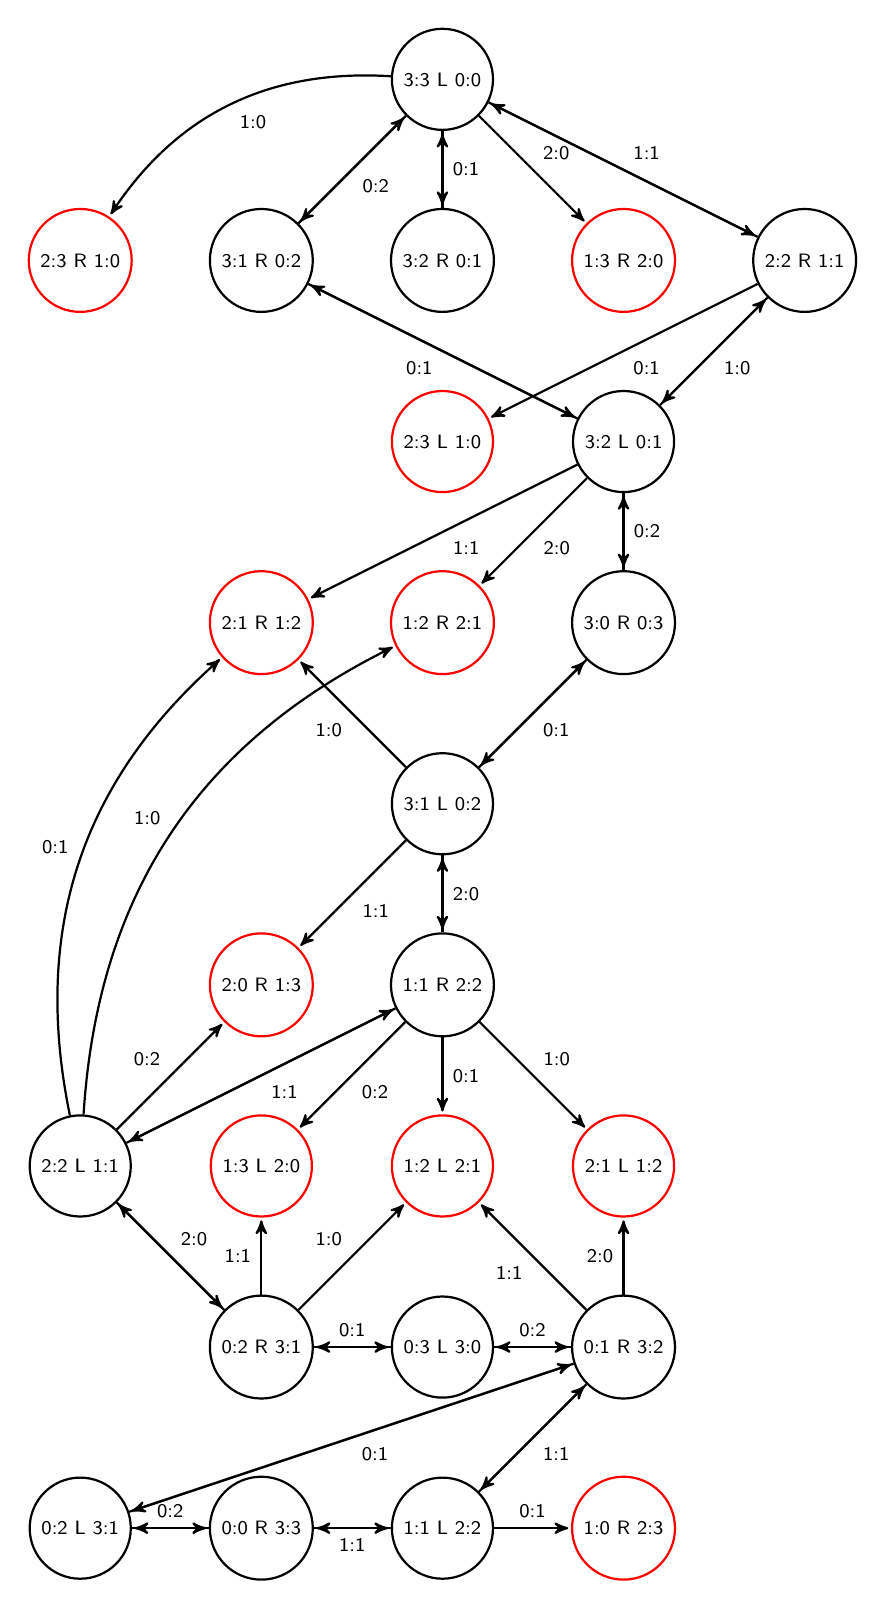
\begin{tikzpicture}[->,>=stealth',shorten >=1pt,auto,node distance=2.3cm,
                    thick,main node/.style={circle,draw,font=\sffamily\scriptsize}]

  \node[main node] (1) {3:3 L 0:0};

  \node[main node] (2) [below of=1] {3:2 R 0:1};
  \node[main node, ] (3) [left of=2] {3:1 R 0:2};
  \node[main node] (4) [left of=3, draw=red] {2:3 R 1:0};
  \node[main node] (5) [right of=2, draw=red] {1:3 R 2:0};
  \node[main node] (6) [right of=5] {2:2 R 1:1};

  \node[main node] (7) [below of=2, draw=red] {2:3 L 1:0};
  \node[main node] (8) [right of=7] {3:2 L 0:1};

  \node[main node] (9) [below of=7, draw=red] {1:2 R 2:1};
  %\node[main node] (10) [left of=9] {3:1 R 0:2};	Repeat of node 3
  \node[main node] (11) [left of=9, draw=red] {2:1 R 1:2};
  \node[main node] (12) [right of=9] {3:0 R 0:3};

  \node[main node] (13) [below of=9] {3:1 L 0:2};

  \node[main node] (14) [below of=13] {1:1 R 2:2};
  \node[main node] (15) [left of=14, draw=red] {2:0 R 1:3};

  \node[main node] (16) [below of=14, draw=red] {1:2 L 2:1};
  \node[main node] (17) [right of=16, draw=red] {2:1 L 1:2};
  \node[main node] (18) [left of=16, draw=red] {1:3 L 2:0};
  \node[main node] (19) [left of=18] {2:2 L 1:1};

  \node[main node] (20) [below of=18] {0:2 R 3:1};
  \node[main node] (21) [right of=20] {0:3 L 3:0};

  \node[main node] (22) [right of=21] {0:1 R 3:2};

  \node[main node] (26) [below of=20] {0:0 R 3:3};
  \node[main node] (23) [left of=26] {0:2 L 3:1};
  \node[main node] (24) [right of=26] {1:1 L 2:2};
  \node[main node] (25) [right of=24, draw=red] {1:0 R 2:3};




  \path[every node/.style={font=\sffamily\scriptsize}]
	(1) edge node {0:1} (2)
		edge node {0:2} (3)
	   	edge [bend right] node {1:0} (4)
	   	edge node {2:0} (5)
	   	edge node {1:1} (6)
	(2) edge node {} (1)
	(3) edge node {} (1)
		edge node {} (8)
	(6) edge node {0:1} (7)
		edge node {1:0} (8)
		edge node {} (1)
	(8) edge node {} (6)
	(8) edge node {2:0} (9)
		edge node {0:1} (3)
		edge node {1:1} (11)
		edge node {0:2} (12)
	%(10) edge node {0:2} (1)
	(12) edge node {0:1} (13)
		edge node {} (8)

	(13) edge node {2:0} (14)
		edge node {1:1} (15)
		edge node {1:0} (11)
		edge node {} (12)

	(14) edge node {0:1} (16)
		edge node {1:0} (17)
		edge node {0:2} (18)
		edge node {1:1} (19)
		edge node {} (13)
		%edge [bend right] node {} (20)

	(19) edge node {2:0} (20)
		edge [bend left] node {0:1} (11)
		edge [bend left] node {1:0} (9)
		edge node {0:2} (15)
		edge node {} (14)
		

	(20) edge node {0:1} (21)
		edge node {1:1} (18)
		edge node {1:0} (16)
		edge node {} (19)

	(21) edge node {0:2} (22)
		edge node {} (20)
		

	(22) edge node {0:1} (23)
		edge node {1:1} (24)
		edge node {2:0} (17)
		edge node {1:1} (16)
		edge node {} (21)

	(23) edge node {0:2} (26)
		edge node {} (22)

	(24)	edge node {0:1} (25)
		edge node {1:1} (26)
		edge node {} (22)

	(26) edge node {} (23)
		edge node {} (24);
	   
\end{tikzpicture}
\section{Implementation of BFS and A* using python}
\begin{verbatim}

from itertools import combinations
from copy import deepcopy
from queue import Queue
from heapq import heappop, heappush

solutions = []
hashTable= {}
SOLUTION = [[0, 0], [3, 3], 'R']

class Tree:

    def __init__(self, state, parent = None, action = None, pathCost = 0):
        self.children = [] # The children of the node 
        self.state = state # The state of the node [[ML, CL], [MR, CR], 'Side boat is on']
        self.parent = parent # The parent of the node
        self.action = action # The action taken to get here
        self.pathCost = pathCost # The cost to get to the node, used for BFS
        # The key version of the node used for the key in a dictionary
        self.key = "{}{}{}{}{}".format(self.state[0][0],
self.state[0][1],self.state[1][0],self.state[1][1],self.state[2])
        # A*
        self.g = -1 # cost to get to the node, used for A*
        self.f = -1 # The cost to get to the node + a guess of how for it 
#needs to go, used for A*

        # A Check if the current state is a solution and add it to solutions if it is
        if state == SOLUTION:
            solutions.append(self)
            return
    
    def getChildren(self):
        '''
        Returns: (Tree[]) The array of children of the current node
        '''
        return self.children
\end{verbatim}
\newpage
\begin{verbatim}
    def createChildren(self):
        '''
        Description: Creates the possible children then returns the result
        Returns: (Tree[]) The array of children of the current node
        '''

        options = ''
        count = 0
        children = []

        # Determines the location of the boat
        if self.state[2] == 'L':
            # Adds 1 or 2 M and C to create the possible options
            # That can be done
            options += min(self.state[0][0], 2) * 'M'
            options += min(self.state[0][1], 2) * 'C'

            # Counts the total number of people on the side
            count = min(self.state[0][0] + self.state[0][1], 2)
        else:
            options += min(self.state[1][0], 2) * 'M'
            options += min(self.state[1][1], 2) * 'C'
            count = min(self.state[1][0] + self.state[1][1], 2)

        # Generates all the choose 1 and choose 2 options from the current state
        comb = set(combinations(options, 1))
        if count > 1:
            comb = comb.union(set(combinations(options, 2)))

        # Sort the options so the order is consistant
        # This is needed because the combinations function produces a random order
        comb = sorted(comb)

        # Go through the combinations and append a new tree node based on the M and C's
        for com in comb:

            m = com.count('M')
            c = com.count('C')

            # Filter out any children that would lead back to the parent state
            if self.action is None or not (m == self.action[0] and c == self.action[1]):
                children.append(Tree(self.move((m, c)), self, (m, c), self.pathCost + 1))

        return children
\end{verbatim}
\newpage
\begin{verbatim}
    def AStarAddAllChildren(self):
        '''
        Description: Used for A*
                     Gets the array of children add adds them to the children array
                     and returns the result
        Returns: (Tree[]) The array of children
        '''
        self.children = self.createChildren()
        return self.children

    def addAllChildren(self):
        '''
        Description: Used for BFS
                     Gets the array of children add adds them to the children array
                     if the current node is a valid node
        '''
        if self.check():
            self.children = self.createChildren()

    def move(self, moves):
        '''
        Description: applies a move to a node
        '''
        newState = deepcopy(self.state)

        if newState[2] == 'L':
            newState[1][0] += moves[0]
            newState[1][1] += moves[1]
            newState[0][0] -= moves[0]
            newState[0][1] -= moves[1]
        else:
            newState[0][0] += moves[0]
            newState[0][1] += moves[1]
            newState[1][0] -= moves[0]
            newState[1][1] -= moves[1]

        newState[2] = 'L' if newState[2] == 'R' else 'R'

        return newState

    def checkValid(self):
        '''
        Description: Checks if a node is valid
        Returns: (Bool) False if C > M at any point True otherwise
        '''
        return not (((self.state[0][0] < self.state[0][1]) and self.state[0][0] != 0) or ((self.state[1][0] < self.state[1][1]) and self.state[1][0] != 0))

    def check(self):
        '''
        Description: Checks if a node is valid and not used
        Returns: (Bool) False if C > M at any point and the node hasn't been used yet True otherwise
        '''
        return self.checkValid() and not self.isInTree()

    def isInTree(self):
        '''
        Description: Checks if the current node has been used (ie is it in the tree)
        Returns: (Bool) True if the node is in the tree, False otherwise
        '''

        value = hashTable.get(self.key)
        if value == None: #value doesn't exist in the table
            hashTable[self.key] = True
            return False

        return True

    def __lt__(self, value):
        return self.f < value.f

    def __str__(self, level=0):
        ret = "\t" * level + repr(self.state) + "\n"
        for child in self.children:
            ret += child.__str__(level + 1)
        return ret

    def __repr__(self):
        return str(self.state) + " " + str(self.f)

def AStar(start):
    '''
    Description: Runs the A* algorithm from the given start node
    Prints: The nodes searched and the optimal solution found
    '''

    frontier = [start]

    checked = {}

    start.f = h(start)
    start.g = 0
\end{verbatim}
\newpage
\begin{verbatim}
    while len(frontier) != 0:

        current = heappop(frontier)

        if current.state == SOLUTION:
            print(start)
            print_solution(current)
            return

        checked[current.key] = True

        for child in current.AStarAddAllChildren():

            if checked.get(child.key):
                continue

            gScore = current.g + 1

            if child.checkValid() and (child.g == -1 or gScore < child.g):

                child.parent = current
                child.g = gScore
                child.f = child.g + h(child)

                if child not in frontier:
                    heappush(frontier, child)
    return None

def h(node):
    '''
    Description: The heuristic for A*
                 h = (number of people on left side) - 1
                 Is admissible because every round trip (boat move to right side then back)
                 results in at most A net of 1 person (except the last move 
	      since at least one person has to return.
    '''
    return node.state[0][0] + node.state[0][1] - 1

def BFS(root):
    '''
    Description: Performs a BFS search from the given start node
    Prints: The nodes searched and the optimal solution found
    '''
    head = Queue()
    head.put(root)
\end{verbatim}
\newpage
\begin{verbatim}
    while (head.empty() is not True ): 
        node = head.get()
        node.addAllChildren()
        
        for child in node.getChildren():
            head.put(child)

    print(root)
    
    for solution in solutions:
        print_solution(solution)
    
def print_solution(end):
    '''
    Description: Prints the solution from the given end point
    Prints: The solution
    '''
    s = []
    
    node = end

    while node is not None:
        s.append(node)
        node = node.parent

    print("=" * 20)
    while len(s) != 0:
        n = s.pop()

        p = "({:3} {:3} | {:3} {:3})[{:1}]".format(n.state[0][0] * 'M', n.state[0][1] * 'C', 
                                                   n.state[1][0] * 'M', n.state[1][1] * 'C', n.state[2])
        print(p)

    print("=" * 20)
    print()

def main():
            # Left side, Right side
            #[[M, C], [M, C], 'Side boat is on']
            # Cost of each action is 1
    print("BFS")
    root = Tree([[3, 3], [0, 0], 'L'])
    BFS(root)
    print("=" * 20)
    print("AStar")
    AStar(Tree([[3, 3], [0, 0], 'L']))

if __name__ == "__main__":
    main()
\end{verbatim}
The output of the code is the optimal solution : \\
Path that each of the algorithms took to find the solution
\begin{verbatim}
BFS
[[3, 3], [0, 0], 'L']
    [[3, 2], [0, 1], 'R']
    [[3, 1], [0, 2], 'R']
        [[3, 2], [0, 1], 'L']
            [[3, 0], [0, 3], 'R']
                [[3, 1], [0, 2], 'L']
                    [[2, 1], [1, 2], 'R']
                    [[2, 0], [1, 3], 'R']
                    [[1, 1], [2, 2], 'R']
                        [[1, 2], [2, 1], 'L']
                        [[1, 3], [2, 0], 'L']
                        [[2, 1], [1, 2], 'L']
                        [[2, 2], [1, 1], 'L']
                            [[2, 1], [1, 2], 'R']
                            [[2, 0], [1, 3], 'R']
                            [[1, 2], [2, 1], 'R']
                            [[0, 2], [3, 1], 'R']
                                [[0, 3], [3, 0], 'L']
                                    [[0, 1], [3, 2], 'R']
                                        [[0, 2], [3, 1], 'L']
                                            [[0, 0], [3, 3], 'R']
                                                [[0, 1], [3, 2], 'L']
                                                [[1, 0], [2, 3], 'L']
                                                [[1, 1], [2, 2], 'L']
                                                [[2, 0], [1, 3], 'L']
                                        [[1, 1], [2, 2], 'L']
                                            [[1, 0], [2, 3], 'R']
                                            [[0, 0], [3, 3], 'R']
                                        [[1, 2], [2, 1], 'L']
                                        [[2, 1], [1, 2], 'L']
                                [[1, 2], [2, 1], 'L']
                                [[1, 3], [2, 0], 'L']
            [[2, 2], [1, 1], 'R']
            [[2, 1], [1, 2], 'R']
            [[1, 2], [2, 1], 'R']
    [[2, 3], [1, 0], 'R']
    [[2, 2], [1, 1], 'R']
        [[2, 3], [1, 0], 'L']
        [[3, 2], [0, 1], 'L']
    [[1, 3], [2, 0], 'R']
====================
AStar
[[3, 3], [0, 0], 'L']
    [[3, 2], [0, 1], 'R']
    [[3, 1], [0, 2], 'R']
        [[3, 2], [0, 1], 'L']
            [[3, 0], [0, 3], 'R']
                [[3, 1], [0, 2], 'L']
                    [[2, 1], [1, 2], 'R']
                    [[2, 0], [1, 3], 'R']
                    [[1, 1], [2, 2], 'R']
                        [[1, 2], [2, 1], 'L']
                        [[1, 3], [2, 0], 'L']
                        [[2, 1], [1, 2], 'L']
                        [[2, 2], [1, 1], 'L']
                            [[2, 1], [1, 2], 'R']
                            [[2, 0], [1, 3], 'R']
                            [[1, 2], [2, 1], 'R']
                            [[0, 2], [3, 1], 'R']
                                [[0, 3], [3, 0], 'L']
                                    [[0, 1], [3, 2], 'R']
                                        [[0, 2], [3, 1], 'L']
                                            [[0, 0], [3, 3], 'R']
                                        [[1, 1], [2, 2], 'L']
                                        [[1, 2], [2, 1], 'L']
                                        [[2, 1], [1, 2], 'L']
                                [[1, 2], [2, 1], 'L']
                                [[1, 3], [2, 0], 'L']
            [[2, 2], [1, 1], 'R']
            [[2, 1], [1, 2], 'R']
            [[1, 2], [2, 1], 'R']
    [[2, 3], [1, 0], 'R']
    [[2, 2], [1, 1], 'R']
        [[2, 3], [1, 0], 'L']
        [[3, 2], [0, 1], 'L']
            [[3, 1], [0, 2], 'R']
            [[3, 0], [0, 3], 'R']
            [[2, 1], [1, 2], 'R']
            [[1, 2], [2, 1], 'R']
    [[1, 3], [2, 0], 'R']
====================

\end{verbatim}
\newpage
Both algorithms produce the same optimal solution
\begin{verbatim}

====================
(MMM CCC |        )[L]
(MMM C   |     CC )[R]
(MMM CC  |     C  )[L]
(MMM     |     CCC)[R]
(MMM C   |     CC )[L]
(M   C   | MM  CC )[R]
(MM  CC  | M   C  )[L]
(    CC  | MMM C  )[R]
(    CCC | MMM    )[L]
(    C   | MMM CC )[R]
(    CC  | MMM C  )[L]
(        | MMM CCC)[R]
====================
\end{verbatim}
\end{document}
